\chapter{Observación microscópica}
Microscopio óptico de campo claro con objetivo de inmersión x100. Los objetivos de 10x y 40x se usan para enfocar los microorganismos. El aumento viene determinado por:
\begin{equation}
	\mbox{Aumento total} = \mbox{Amplitud ocular} \cdot \mbox{Amplitud objetivo}
\end{equation}
Se suele conseguir entre 1000x y 1500x aumentos si se utiliza aceite de cedro con el objetivo de inmersión; en caso contrario, no se ve nada, es decir, poco definido.
\begin{equation}
	d = \frac{0.5 \cdot \lambda}{N\cdot \sin \theta}
\end{equation}
Donde:
\begin{description}[itemsep=0pt,parsep=0pt,topsep=0pt,partopsep=0pt]
	\item[d]: es la distancia entre dos puntos como entidades separadas.
	\item[$\lambda$]: es la longitud de onda del haz de electrones.
	\item[$N \sin\theta$] es la apertura numérica del diafragma, siendo $N$ a su vez el índice de refracción de una sustancia. El índice de refracción del aire es de 1, mientras que el del aceite es de 1.2 a 1.4. Con esto se mejora la resolución y se ven los microorganismos más nítidos.
\end{description}
\section{Preparaciones}
\begin{enumerate}[itemsep=0pt,parsep=0pt,topsep=0pt,partopsep=0pt]
	\item \textbf{Fijación al porta} (al lavar sin fijar se pierden todos los microorganismos). 
	\begin{enumerate}[itemsep=0pt,parsep=0pt,topsep=0pt,partopsep=0pt]
		\item Para eso antes se debe realizar un frotis. Sobre un porta se coloca una gota de agua. Sobre esa gota se resuspende el microorganismo gracias al asa de siembra.
		\item Uso del asa de siembra: Siempre debe manejarse en condiciones de total esterilidad. Se debe mantener siempre el mechero encendido y regular el paso de gas hasta obtener una llama no muy grande y azulada. Se pasa el filamento metálico del asa de siembra por la llama para volverlo incandescente antes y después de la aplicación. Al coger los microorganismos del tubo también se debe flambear el tubo una fracción de segundo.
		\item Se extiende por el porta y se deja secar al aire (lento), o sobre la llama del mechero (rápido).
	\end{enumerate}
	\item \textbf{Tinción}: Las tinciones pueden ser de tres tipos:
	\begin{itemize}[itemsep=0pt,parsep=0pt,topsep=0pt,partopsep=0pt]
		\item \textit{\textbf{Simples}}: Directas, Negativas.
		\item \textit{\textbf{Diferenciales}}.
		\item \textit{\textbf{Especiales}}.
	\end{itemize}
	Las tinciones simples directas se realizan con colorantes básicos o catiónicos (azul de metileno, safranina, etc). Con estas tinciones penetrantes se distingue tanto la forma del microorganismo como las agrupaciones. No penetran en el microorganismo las tinciones ácidas, aniónicas o negativa. En ellas también se ve muy bien la ultraestructura bacteriana y las agrupaciones, puesto que solo se tiñe el fondo de la preparación.
\end{enumerate}
\begin{table}[H]
	\centering
	\begin{tabular}{c c}
		\rowcolor{black}\textcolor{white}{\textbf{Tinciones positivas}}&\textcolor{white}{\textbf{Tinciones negativas}}\\
		Preparación de un frotis, que será fijado.&El microorganismo se resuspende en el propio colorante,\\
		\rowcolor{hiperlightgray}Cubrir con colorante de 2-5 minutos.& y en esa gota se resuspende y extiende.\\
		Lavar con agua y poner en la rejilla.&No se lava con agua, y tampoco se fija el frotis\\
		\rowcolor{hiperlightgray}Escurrir al aire con el porta inclinado.&Mejor visión: Al no fijar el frotis no se deshidrata\\
		\hline
	\end{tabular}
	\caption{Diferencias entre tinciones positivas y tinciones negativas}
\end{table}
\section{Tinciones diferenciales}
Las tinciones diferenciales tiñen en función de las características del microorganismo. Constan siempre de dos colorantes.
\subsection{Tinción de Gram}
Importantísima tinción diferencial para diferenciar bacterias Gram positivas de Gram negativas. Dependerá de la estructura de la pared celular.
\begin{enumerate}[itemsep=0pt,parsep=0pt,topsep=0pt,partopsep=0pt]
	\item Hacer un frotis.
	\item Tinción propiamente dicha:
	\begin{enumerate}[itemsep=0pt,parsep=0pt,topsep=0pt,partopsep=0pt]
		\item Cristal violeta (2 min). Tiñe todos los microorganismos.
		\item Decántese el exceso y añadimos lugol (1 min). Este lugol se une al cristal violeta formando el complejo lugol-cristal violeta. Aumenta el tamaño de la molécula de forma considerable.
		\item Decolorar con etanol 96º 30 segundos tres veces. En función de la pared celular el alcohol va a arrastrar, o no, el anterior complejo fuera. 
		\item Lavar con agua destilada.
		\item Safranina 1 min. Tiñe los microorganismos decolorados.
		\item Lávese con agua destilada de nuevo.
		\item Secado al aire con el porta inclinado.
	\end{enumerate}
	\item Observación
\end{enumerate}
Funcionamiento a nivel molecular y macromolecular:
\begin{itemize}[itemsep=0pt,parsep=0pt,topsep=0pt,partopsep=0pt]
	\item Gram positivas (\textit{Staphylococcus aureus, Streptococus thermophilus}) Agrupación en racimo de uva y en cadenas, respectivamente:
	\begin{itemize}[itemsep=0pt,parsep=0pt,topsep=0pt,partopsep=0pt]
		\item Pasa el cristal violeta
		\item Pasa el lugol y se forma el complejo cristal violeta-lugol
		\item El alcohol contrae el peptidoglucano y la malla se vuelve más tupida. Por mucho alcohol de más que yo le eche, el complejo cristal violeta-Lugol no puede salir.
		\item La safranina no puede teñir nada.
	\end{itemize}
	\item Gram negativos (\textit{Escherichia coli)}
	\begin{itemize}[itemsep=0pt,parsep=0pt,topsep=0pt,partopsep=0pt]
		\item Pasa el cristal violeta.
		\item Pasa el lugol.
		\item El etanol elimina la membrana externa y contrae el peptidoglucano. Puesto que la malla es muy poco tupida el complejo cristal violeta-Lugol se va.
		\item La safranina teñirá entonces de color rojizo-rosáceo las bacterias.
	\end{itemize}
\end{itemize}
La célula vegetativa aparece teñida, y la endospora aparece sin teñir, pues no capta los colorantes básicos. La mayoría de las preparaciones analizadas serán de cultivo mixto, con muchos tipos de bacterias.
\subsection{Tinción ácido-alcohol resistente} 
Tinción diferencial que permite observar bacterias por la estructura de su pared (\textit{Mycobacterium}, \textit{Nocordia}). Se debe recordar que en las Gram positivas la pared estaba compuesta en un 90\% de peptidoglucano. No obstante, había algunas bacterias con menos peptidoglucano pero con ácidos micólicos, ácidos grasos de cadena larga que impiden una correcta tinción por métodos convencionales. Esta tinción utiliza dos colorantes:
\begin{itemize}[itemsep=0pt,parsep=0pt,topsep=0pt,partopsep=0pt]
	\item \textbf{Colorante primario}: fucsina fenicada (contiene fenol). Las ceras son hidrófobas y el fenol penetra bien por ahí. Se mantiene cinco minutos con calor. Este puede ser proporcionado por un hisopo (vidrio con algodón en la punta). Cuando empiecen a emitirse vapores se debe retirar el porta. 
	\item \textbf{Decolorante}: etanol + HCl. (alcohol ácido)
	\item \textbf{Colorante secundario}: azul de metileno (1 minuto). Lavar con agua y secado inclinado.
\end{itemize}

Si el alcohol ácido ha sido capaz de decolorar el microorganismo, estos se verán teñidos de azul. La capa cérea repele el alcohol ácido y solo se tiñe con fucsina, luego es ácido alcohol resistente. Lo que se espera hallar es la presencia en esputos de bacterias como \textit{M. tuberculosis} o \textit{M. lepre}. Observar en la imagen correspondiente a esta tinción bacilos alargados del género \textit{Mycobacterium} teñidos de color rosa. Se dice, por tanto, que esa muestra es positiva para esta tinción. 
\subsection{Tinciones específicas de endospora}
\begin{enumerate}[itemsep=0pt,parsep=0pt,topsep=0pt,partopsep=0pt]
	\item Para las endosporas  se obtiene un frotis normal y se tiñe posteriormente con verde malaquita con la ayuda de un papel de filtro. Mantener 8 minutos calentando de forma intermitente hasta la emisión de vapores. El verde malaquita penetra en este proceso. 
	\item Lavar con agua destilada.
	\item Añadir safranina, 1 minuto. Lavar con agua y escurrir con el porta inclinado al aire.
	\item Se puede ver:
	\begin{itemize}[itemsep=0pt,parsep=0pt,topsep=0pt,partopsep=0pt]
		\item Células teñidas solo de verde (endosporas)
		\item Células teñidas de rosa (célula vegetativa)
	\end{itemize}
\end{enumerate}
En un mismo cultivo se pueden ver todos los elementos: endosporas libres, células vegetativas lisadas, células vegetativas con endospora dentro…
\subsection{Tinciones específicas de cápsula}
Frotis con tinta china y safranina, o con tinta china a secas. Es una tinción similar a las simples negativas. La bacteria será teñida por la tinta y la cápsula no se tiñe.
\subsection{Tinción de Ryu o de flagelos}
\begin{itemize}[itemsep=0pt,parsep=0pt,topsep=0pt,partopsep=0pt]
	\item Gota de agua en el porta
	\item Deposición de la colonia.
	\item Engrosar el flagelo con una preparación a base de fenol, ácido tánico y alumbre. Mezclar en proporción 1:1 con otra solución de cristal violeta para visualizar el flagelo. La tinción dura 7 min y después se ha de lavar con agua destilada unos dos minutos.
\end{itemize}
\begin{figure}[H]
	\centering
	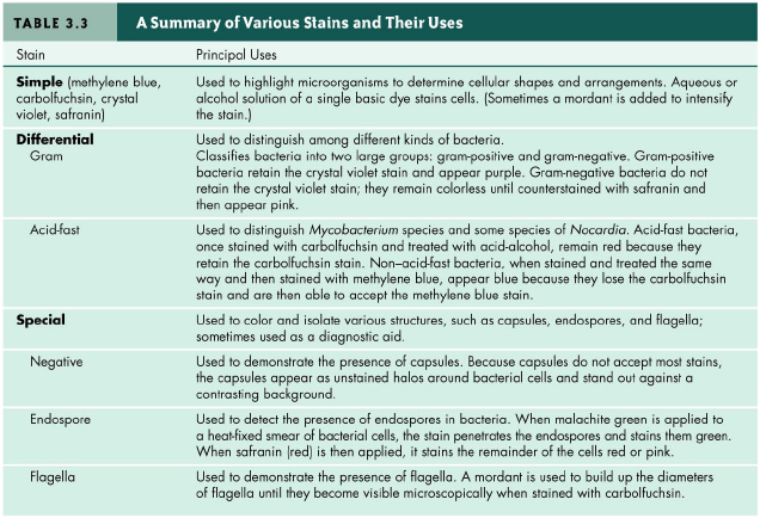
\includegraphics[width=\columnwidth]{A.imagenes/ACV-MICRO-Temp1}
	\caption[Resumen de las principales tinciones.]{Resumen de las principales tinciones. \textit{\textbf{Extraido de:}} \cite{Prescott2011}}
\end{figure}